\documentclass[10pt]{exam}
\usepackage[hon]{template-for-exam}
\usepackage{circuitikz}


\title{Equivalent Resistance}
\author{Rohrbach}
\date{\today}

\begin{document}
\maketitle

\begin{questions}

\question
  \textbf{Consolidation:} Find the current going through the battery in the circuit below.
  
  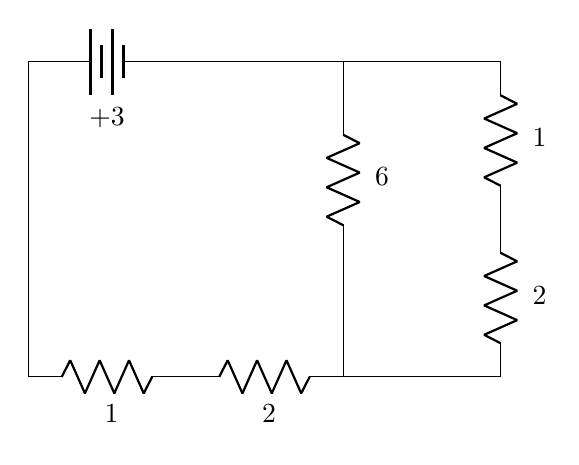
\begin{tikzpicture}
    \draw (0,0) 
      to                     ++(0,4)
      to[battery,l_=$+\SI{ 3}{\volt}$] ++(2,0)
      to                     ++(2,0) coordinate (a)
      to[R,l=\SI{  6}{\ohm}] ++(0,-3)
      to                     ++(0,-1) coordinate (b)
      to[R,l=\SI{  2}{\ohm}] ++(-2,0)
      to[R,l=\SI{  1}{\ohm}] ++(-2,0);
    \draw (a)
      to                     ++(2,0)
      to[R,l=\SI{  1}{\ohm}] ++(0,-2)
      to[R,l=\SI{  2}{\ohm}] ++(0,-2)
      to (b);
  \end{tikzpicture}

  \vs


\question
  Find the current going through the battery in the circuit below.
  
  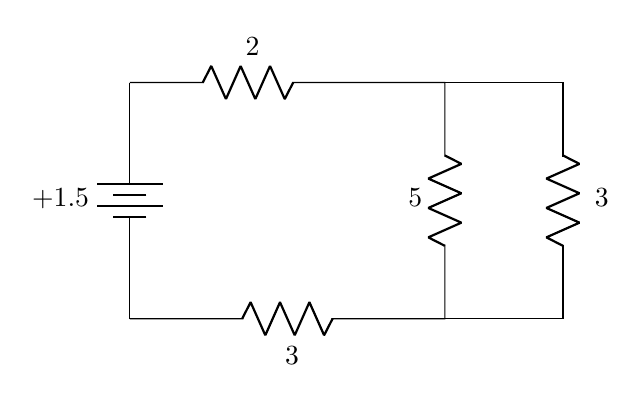
\begin{tikzpicture}
    \draw (0,3)
      to[battery,l_=$+\SI{ 1.5}{\volt}$] (0,0);
    \draw (0,3) 
      to[R,l=\SI{ 2}{\ohm}]  ++(3, 0)
      to                     ++(1, 0) coordinate (a)
      to[R,l_=\SI{  5}{\ohm}] ++(0,-3) coordinate (b)
      to[R,l=\SI{  3}{\ohm}] ++(-4,0);
    \draw (a)
      to                     ++(1.5,0)
      to[R,l=\SI{  3}{\ohm}] ++(0,-3) 
      to                       (b);
  \end{tikzpicture}

  \vs 

\pagebreak

\question \label{1}
  Find the current going through the battery in the circuit below.
  
  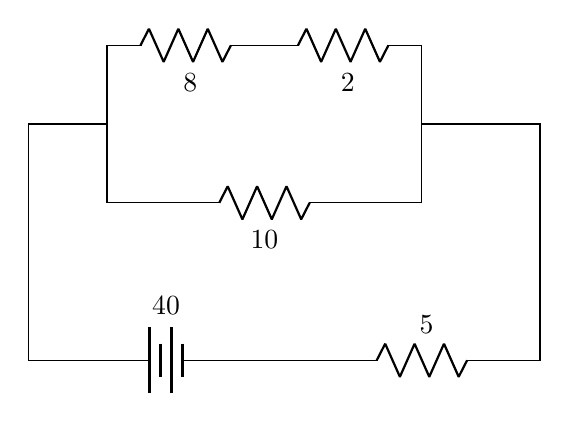
\begin{tikzpicture}
    \draw (0,0)
      to[battery,l=\SI{40}{\volt}] 
                                  ++(3.5,0)
      to[R,l=\SI{ 5}{\ohm}]       ++(3,0)
      to                          ++(0,3)
      to                          ++(-1.5,0)
                                   coordinate (a)
      to                          ++(0,1)
      to[R,l=\SI{ 2}{\ohm}]       ++(-2,0)
      to[R,l=\SI{ 8}{\ohm}]       ++(-2,0)
      to                          ++(0,-1) coordinate (b)
      to                          ++(-1,0)
      to                          ++(0,-3);
    \draw (a) to                  ++(0,-1)
      to[R,l=\SI{10}{\ohm}]       ++(-4,0) to (b);
  \end{tikzpicture}

  \vs
  

\question \label{2}
  Find the current going through the battery in the circuit below.
  
  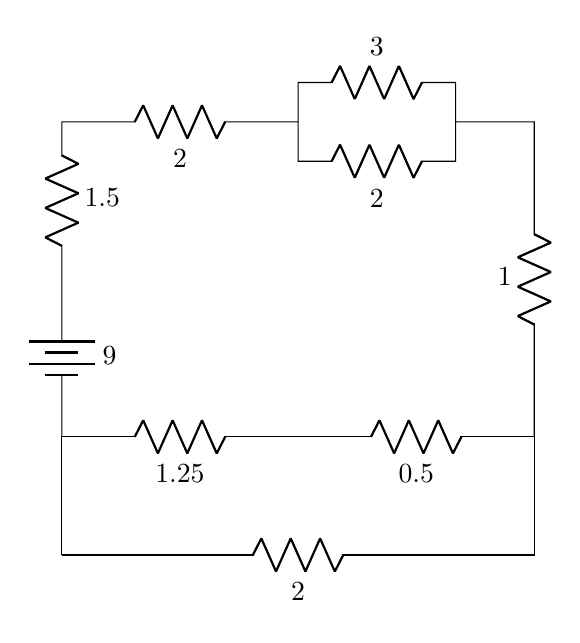
\begin{tikzpicture}
    \draw (0,0) 
      to[R,l_=\SI{2}{\ohm}]      ++( 6, 0)
      to                         ++(0,1.5) coordinate (b)
      to[R,l=\SI{0.5}{\ohm}]     ++(-3, 0)
      to[R,l=\SI{1.25}{\ohm}]    ++(-3, 0) coordinate (a)
      to                         ++( 0,-1.5);
    \draw (b)
      to[R,l=\SI{1}{\ohm}]     ++( 0, 4)
      to                       ++(-1, 0)   coordinate (c)
      to                       ++( 0,0.5)
      to[R,l_=\SI{3}{\ohm}]    ++(-2, 0)
      to                       ++( 0,-0.5) coordinate (d)
      to[R,l=\SI{2}{\ohm}]     ++(-3,0)
      to[R,l=\SI{1.5}{\ohm}]   ++(0,-2)
      to[battery,l=\SI{9}{\volt}] ++(0,-2);
    \draw (c)
      to                       ++(0,-0.5)
      to[R=\SI{2}{\ohm}]       ++(-2,0)
      to (d);
  \end{tikzpicture}

  \vs


{\footnotesize Answers: \hspace{3em} \ref{1}) \SI{4.00}{\ampere} \hspace{3em} \ref{2}) \SI{1.36}{\ampere} \hfill}

\pagebreak

\question
  Consider the following circuit, in which 
  $R_1 = R_3 = R_5 = R_6 = \SI{1}{k\ohm}$ and
  $R_2 = R_4 = \SI{2}{k\ohm}$.

  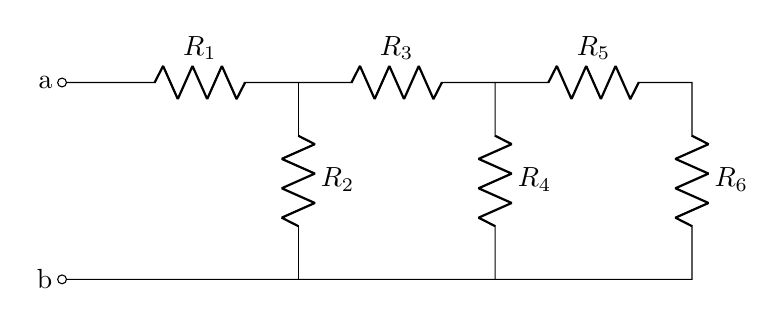
\begin{tikzpicture}
    \draw (0,0)                  coordinate (a)
      to[short,o-] ++( 0.5,   0) coordinate (0)
      to[R=$R_1$]  ++( 2.5,   0) coordinate (1)
      to[R=$R_3$]  ++( 2.5,   0) coordinate (3)
      to[R=$R_5$]  ++( 2.5,   0)
      to[R=$R_6$]  ++(   0,-2.5)
      to[short,-o] ++(-8.0,   0) coordinate (b);
    \draw (1) to[R=$R_2$] ++(0,-2.5);
    \draw (3) to[R=$R_4$] ++(0,-2.5);
    \node[anchor=east] at (a) {a};
    \node[anchor=east] at (b) {b};
  \end{tikzpicture}


  \begin{parts}
    \part Calculate Equivalent Resistance
    \part A 9-volt battery is connected between points $a$ and $b$.  Calculate the current through \emph{each} resistor.
    \part Calculate the potential difference across each resistor.
  \end{parts}

\pagebreak

\question
  \textbf{Bonus:} Calculate the equivalent resistance of a cube that has a 1-ohm resistor along each edge.

  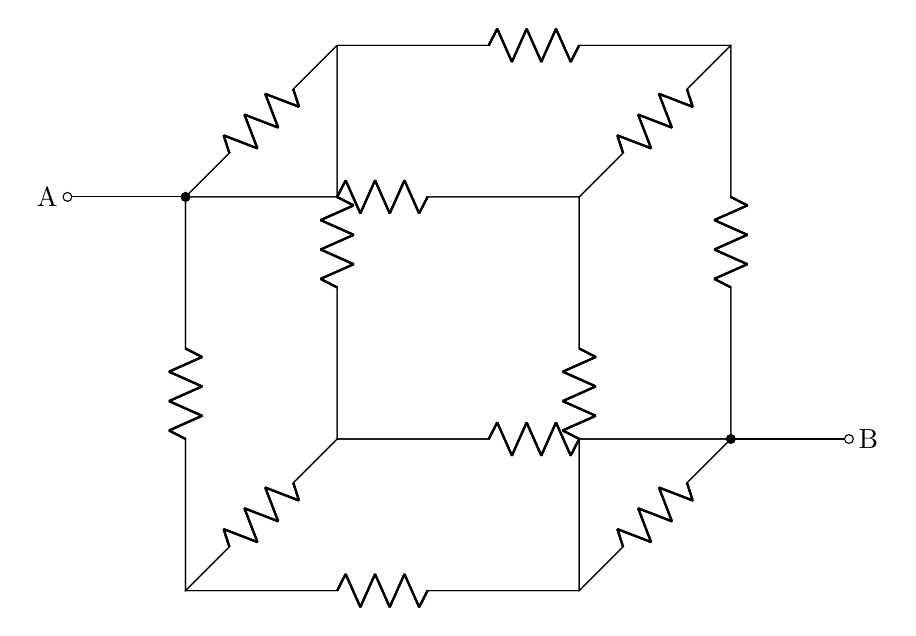
\begin{tikzpicture}
    \def\s{5}
    \coordinate (A) at (0,0,0);
    \coordinate (B) at (\s,0,0);
    \coordinate (C) at (\s,\s,0);
    \coordinate (D) at (0,\s,0);
    \coordinate (E) at (0,0,\s);
    \coordinate (F) at (\s,0,\s);
    \coordinate (G) at (\s,\s,\s);
    \coordinate (H) at (0,\s,\s);
    
    % Draw the cube
    \draw (A) to[R] (B) to[R] (C) to[R] (D) to[R] (A);
    \draw (A) to[R] (E) to[R] (F) to[R] (B) to[R] (A);
    \draw (B) to[R] (F) to[R] (G) to[R] (C) to[R] (B);
    \draw (C) to[R] (G) to[R] (H) to[R] (D) to[R] (C);
    \draw (D) to[R] (H) to[R] (E) to[R] (A) to[R] (D);
    \draw (E) to[R] (H) to[R] (G) to[R] (F) to[R] (E);
    \draw (H) to[short, *-o] ++(-1.5,0) node[left] {A};
    \draw (B) to[short, *-o] ++(1.5,0) node[right] {B};

    
  \end{tikzpicture}


\end{questions}

\pagebreak

\end{document}